\section{Discussion of individual modules}
\label{sec:noah__modules}

The GENESIS website makes it possible to easily implement and distribute entirely new modules, as well as updates to old modules: simply changing the underlying \texttt{NOAHModule} objects is sufficient to propagate changes to all supersequences generated using those modules.
In this section, I discuss a number of new pulse sequence developments made in the course of my DPhil; all of these have been successfully implemented in GENESIS and are available to download.

With regards to sensitivity analyses, since this chapter discusses the design of \textit{individual modules}, I have chosen to focus almost entirely on the SNR factor $A$: this is an intrinsic property of the module.
In contrast, the quantities $\rho_t$ and $\varepsilon_t$ depend on the supersequence within which the module is used, and can be improved trivially by adding more modules to the supersequence under consideration.
These numbers reflect the utility of the NOAH \textit{technique}, but are not relevant to the individual modules from which they are constructed.

\subsection{\texorpdfstring{\carbon{}}{13C} sensitivity-enhanced HSQC}
\label{subsec:noah__sehsqc_c}

The first new module is the sensitivity-enhanced HSQC (seHSQC) experiment, which provides up to $2\times$ increased SNR over a standard (echo--antiecho) HSQC.%
\footnote{Since a States HSQC has $\sqrt{2}$ times the SNR of an EA HSQC (as shown in \cref{fig:hsqc_comparison}), this also means that the seHSQC has a $\sqrt{2}$ SNR improvement over a States HSQC. The literature can be somewhat confusing on this point: sometimes the gain in signal is even conflated with the gain in SNR. The clearest exposition I have found is that provided by Kontaxis et al.\autocite{Kontaxis1994JMRSA}}
In the original version of the seHSQC (\cref{fig:sehsqc_po_crk}), developed by Cavanagh, Rance, and Kay (`CRK')\autocite{Palmer1991JMR,Kay1992JACS}, this is accomplished through the so-called \textit{preservation of equivalent pathways} (PEP) technique\autocite{Cavanagh1993ARNMRS}, which I now provide a product operator analysis of.

\begin{figure}[!htbp]
    \centering
    
\includegraphics[]{pp/sehsqc/all_po.png}%
    {\phantomsubcaption\label{fig:sehsqc_po_crk}}%
    {\phantomsubcaption\label{fig:sehsqc_po_noah1}}%
    {\phantomsubcaption\label{fig:sehsqc_po_noah2}}%
    \caption[CRK seHSQC and NOAH seHSQC modules]{
        Sensitivity-enhanced HSQC sequences discussed in this section, along with product operator analysis.
        This analysis is provided only for the first step of the phase cycle, and assumes an $IS\/$ spin pair with $\Delta' = 1 / (4 \cdot \oneJ{CH})$.
        `cos \magn{C}' refers to the component of the \magn{C} magnetisation which is cosine-modulated during $t_1$.
        \textbf{(\subref*{fig:sehsqc_po_crk})} Cavanagh--Rance--Kay seHSQC.
        \textbf{(\subref*{fig:sehsqc_po_noah1})} NOAH seHSQC1 module.
        \textbf{(\subref*{fig:sehsqc_po_noah2})} NOAH seHSQC2 module.
        Phase cycling is performed with $\phi_1 = (x, -x)$, $\phi_2 = (x, x, -x, -x)$, and $\phirec = (x, -x, -x, x)$.
        The delay $\Delta$ is set to $1 / (4 \cdot \oneJ{CH})$; see the text for a discussion of $\Delta'$.
        A value of \qty{145}{\Hz} was used for $\oneJ{CH}$.
        The pulses marked with a phase of $\pm y\/$ are applied with a phase of $y\/$ in the echo experiment and $-y\/$ in the antiecho.
        Gradient amplitudes are $(g_1, g_2, g_2', g_3, g_4) = (70\%, \pm 35.2\%, \pm 17.6\%, 11\%, -5\%)$.
    }
    \label{fig:sehsqc_po}
\end{figure}

Just like in a standard HSQC, the seHSQC experiment begins with an INEPT block and $t_1$ evolution.
At the end of $t_1$, there are two terms which are cosine- and sine-modulated with respect to $\Omega_S$.
In the standard HSQC, only the $2I_zS_y$ term is returned into observable \proton{} magnetisation by the reverse INEPT block (see \cref{subsec:theory__hsqc_states}).
In contrast, the PEP block transfers \textit{both} terms back to \proton{} and subsequently detects both.
Specifically, in the echo experiment it accomplishes the transfer $2I_zS_y \to I_y$ and $2I_zS_x \to I_x$, meaning that the density operator at the end of $t_1$
\begin{equation}
    \label{eq:sehsqc_t1_modulation}
    -2I_zS_y \cos(\Omega_S t_1) - 2I_zS_x \sin(\Omega_S t_1)
\end{equation}
is transformed into
\begin{equation}
    \label{eq:sehsqc_before_detection}
    -I_y \cos(\Omega_S t_1) - I_x \sin(\Omega_S t_1)
\end{equation}
just prior to acquisition.
During the FID, only the $-1$-coherence component of this is detected:
\begin{equation}
    \label{eq:sehsqc_detection_minusone}
    \frac{1}{2\mi}I_- \cos(\Omega_S t_1) - \frac{1}{2}I_- \sin(\Omega_S t_1) = \frac{1}{2\mi}I_-\exp(-\mi \Omega_S t_1),
\end{equation}
yielding a signal of
\begin{equation}
    \label{eq:s_echo_sehsqc}
    \frac{1}{2\mi}\exp(-\mi \Omega_S t_1)\exp(\mi \Omega_I t_2),
\end{equation}
which has a $2\times$ larger amplitude than the original EA HSQC (\cref{eq:hsqc_ea_echo_signal}).
The antiecho experiment can be similarly analysed.
Since the seHSQC has the same noise level as in an EA HSQC, this also corresponds to a $2\times$ increase in SNR.

It should, however, be noted that the PEP transfer is only fully attained for $IS\/$ spin pairs if the delay $\Delta'$ is set to $1 / (4 \cdot \oneJ{CH})$.
For $I_2S\/$ or $I_3\/S$ spin systems, no gain in sensitivity is accomplished with this setting of $\Delta' = 1 / (4 \cdot \oneJ{CH})$.
It is more common, therefore, to shorten $\Delta'$ to $1 / (8 \cdot \oneJ{CH})$: this sacrifices some transfer efficiency for $IS\/$ systems, but allows for some sensitivity enhancement for $I_2S\/$ and $I_3S\/$ systems (\cref{tbl:sehsqc_theory}).

\begin{table}[!ht]
    \begin{tabular}{cccc}
        \toprule
        \textbf{Spin system} & \multicolumn{3}{c}{\textbf{Theoretical sensitivity enhancement}} \\
        \cmidrule(lr){2-4}
                             & $\Delta' = 1 / (4 \cdot \oneJ{CH})$ & $\Delta' = 1 / (8 \cdot \oneJ{CH})$ & $\Delta' = 1 / (12 \cdot \oneJ{CH})$ \\
        \midrule
        $IS$   & 2 & 1.71 & 1.5  \\
        $I_2S$ & 1 & 1.41 & 1.37 \\
        $I_3S$ & 1 & 1.21 & 1.25 \\
        \bottomrule
    \end{tabular}
    \caption[Theoretical sensitivity enhancements in the seHSQC]{
        Theoretical sensitivity enhancements for $IS\/$, $I_2S\/$, and $I_3S\/$ spin systems in the seHSQC, as a function of the delay $\Delta'$.
        The values are taken from Schleucher et al.\autocite{Schleucher1994JBNMR}
    }
    \label{tbl:sehsqc_theory}
\end{table}


\subsubsection{NOAH seHSQC versions}

Just like the original EA HSQC (\cref{fig:hsqc_etgp}), the CRK seHSQC must be modified in order to be compatible with NOAH supersequences.
In particular, the CTP gradients in the CRK seHSQC dephase the bulk \magnnot{C} magnetisation pool: we would very much like it to return that to $+z$ instead, so that it can be sampled in later homonuclear modules (or, indeed, a HMBC module).
This experiment is more tricky to adapt than the HSQC, because there are \textit{three} different magnetisation components to juggle: the cosine-modulated \magn{C}, sine-modulated \magn{C}, and \magnnot{C}.
Nevertheless, there are at least two ways of doing so; these two modified modules are labelled seHSQC1 and seHSQC2 respectively.

The seHSQC1 module (\cref{fig:sehsqc_po_noah1}) was developed by me.\footnote{Through a great deal of trial and error, and certainly \textit{not} intelligent design.}
It retains the same general structure of the CRK seHSQC up until $t_1$, but immediately after $t_1$ a composite \proton{} pulse is used to effect the transformations
\begin{equation}
    \label{eq:sehsqc1_dp}
    I_z \to I_y; \qquad I_y \to I_x,
\end{equation}
where the former is required for the \magn{C} pool and the latter for \magnnot{C}.
This has the effect of storing the sine-modulated term as $2I_zS_z$ magnetisation for one spin echo (as opposed to the CRK seHSQC, which stores the cosine-modulated term as $I_z$).
At the beginning of the final spin echo, this is transformed into antiphase magnetisation of the form $2I_xS_z$; thus, this spin echo must be lengthened to a total duration of $2\Delta$ in order to fully refocus $\oneJ{CH}$.
The final modification involves the addition of an extra gradient immediately before $t_1$: this ensures that the bulk \magnnot{C} magnetisation is not dephased, just like in the NOAH HSQC module (\cref{fig:noah_sb_po_s}).

The seHSQC2 module (\cref{fig:sehsqc_po_noah2}), on the other hand, was first developed by Hansen et al.\autocite{Hansen2021AC}
In this pulse sequence, the initial \proton{} \angang{90}{x} excitation pulse is replaced with a $zz$ isotope-selective pulse (ZIP) element, which is very similar to the $zz$-filter but has different pulse phases.
The effect of this on the \magn{C} magnetisation pool amounts to a \angang{90}{-x} pulse, and thus the same signals are ultimately detected from this magnetisation pool (save for a trivial \ang{180} phase shift).
However, on \magnnot{C} magnetisation, the ZIP element acts as a \angang{90}{y} pulse; it turns out that this modification alone is sufficient to return the bulk \magnnot{C} magnetisation to $+z$ at the end of the sequence.
The ZIP element therefore represents an \textit{isotope-specific rotation} on protons, where the rotation axis depends on whether the proton is directly coupled to \carbon{} or not.

\begin{figure}[!ht]
    \centering
    
\includegraphics[]{pp/sehsqc/grad_schemes.png}%
    {\phantomsubcaption\label{fig:sehsqc_grad_schemes_alex}}%
    {\phantomsubcaption\label{fig:sehsqc_grad_schemes_jon}}%
    \caption[Comparison of gradient schemes in seHSQC2 module]{
        Comparison of CTP gradient schemes in seHSQC2 module.
        \textbf{(\subref*{fig:sehsqc_grad_schemes_alex})} As reported in Hansen et al.\autocite{Hansen2021AC} $g_0$ is a purge gradient with arbitrary amplitude; the amplitude of the final CTP gradient must be halved.
        \textbf{(\subref*{fig:sehsqc_grad_schemes_jon})} The version used in this work (corresponding to \cref{fig:sehsqc_po_noah2}).
    }
    \label{fig:sehsqc_grad_schemes}
\end{figure}

In my work, I made one change to the experiment, namely the addition of an extra gradient echo prior to $t_1$ (thus leading to a symmetric gradient scheme similar to that in seHSQC1).
Instead of this, the original paper had in fact inserted a purge gradient between the \proton{} and \carbon{} \ang{90} pulses just after the INEPT spin echo (\cref{fig:sehsqc_grad_schemes}).
The scheme I used leads to similar results, but has one advantage in that it allows the amplitude of the final CTP gradient ($g_2$ in \cref{fig:sehsqc_po}) to be twice as large: this is particularly relevant to \nitrogen{} experiments, as will be discussed in \cref{subsec:noah__hmqc}.

\begin{figure}[!ht]
    \centering
    \includegraphics[]{noah/sehsqc_comp.png}%
    {\phantomsubcaption\label{fig:noah_sehsqc_comp_crk}}%
    {\phantomsubcaption\label{fig:noah_sehsqc_comp_v1}}%
    {\phantomsubcaption\label{fig:noah_sehsqc_comp_v2}}%
    \caption[Comparison of \noah{Sp,Cc} sensitivities]{
        Sensitivities of seHSQC and CLIP-COSY modules in the \noah{Sp,Cc} supersequences (run using $\Delta' = 1 / (8 \cdot \oneJ{CH})$).
        Intensities are reported relative to the corresponding peaks in a \noah{S,Cc} supersequence; HSQC peaks are further broken down by their multiplicity.
        Each dot represents one peak; the solid lines as well as the numbers at the bottom of each plot represent averages over all peaks.
        \textbf{(\subref*{fig:noah_sehsqc_comp_crk})} Using the CRK seHSQC.
        \textbf{(\subref*{fig:noah_sehsqc_comp_v1})} Using the seHSQC1 module.
        \textbf{(\subref*{fig:noah_sehsqc_comp_v2})} Using the seHSQC2 module.
        \datacode{7A-201115}
    }
    \label{fig:noah_sehsqc_comp}
\end{figure}

The primary consideration when evaluating the different seHSQC versions in \cref{fig:sehsqc_po} is naturally sensitivity.
\Cref{fig:noah_sehsqc_comp} compares the sensitivities of the various possible \noah{Sp,Cc} supersequence, against a \noah{S,Cc} experiment.
As can be seen, all three seHSQC implementations yield improvements in the sensitivities of \ch{CH} peaks: the original CRK seHSQC has the largest effect here, followed by seHSQC2 and seHSQC1.
For \ch{CH2} and \ch{CH3} peaks, the CRK seHSQC and seHSQC2 perform better than the standard HSQC, but the relative sensitivities in seHSQC1 have dipped slightly below 1.
This is not entirely surprising in light of the discussion in \cref{subsec:noah__snr}: the modified seHSQC1 and seHSQC2 sequences are expected to have lower sensitivities than the original experiment from which they are derived.
In this case, it appears that the modifications made to the seHSQC1 sequence cause sensitivity losses which outweigh the benefits of using a sensitivity-enhanced experiment.

In the context of a NOAH supersequence, it is also important to consider how well each module preserves \magnnot{C} magnetisation for subsequent homonuclear module(s).
In \cref{fig:noah_sehsqc_comp}, the CLIP-COSY module is used as the `reporter' module, but the conclusions drawn here are applicable to \textit{any} homonuclear module (or the HMBC).
The CRK seHSQC does poorly in this respect, as it dephases the bulk magnetisation: this leads to almost an order-of-magnitude sensitivity loss in the CLIP-COSY.
Both the other NOAH seHSQC modules, however, perform almost identically to the original HSQC module, as expected from the product operator analysis in \cref{fig:sehsqc_po}.

From \cref{fig:noah_sehsqc_comp}, we can draw some very simple conclusions: if the seHSQC is to be used at (or near) the \textit{beginning} of a NOAH supersequence, where it needs to preserve \magnnot{C} magnetisation, then the seHSQC2 module is the best choice.
On the other hand, if the seHSQC module is placed at the \textit{end} (say in a \noah{B,Sp} supersequence), then the CRK seHSQC is optimal.
This logic is used by GENESIS to choose the best seHSQC implementation based on other modules in the requested supersequence.


\subsubsection{COSY-type artefacts}

One (minor) way in which the seHSQC1 module outperforms seHSQC2 is in the suppression of COSY-type artefacts in the seHSQC spectrum\autocite{Turner1999JMR}.
These arise due to evolution of $\nJ{HH}$ during the second-last spin echo of the CRK seHSQC.
Specifically, if we assume the presence of a separate \proton{} spin $K$ which is coupled to spin $I$, the sine-modulated $2I_yS_z$ term can evolve under both $\oneJ{$IS$}$ and $\nJ{$IK$}$ into $2I_yK_z$, and the last \proton{} \ang{90} pulse transfers this coherence to the spin $K$.
This leads to peaks correlating spin $S$ with spin $K$.
Since the seHSQC2 module shares the same product operator analysis as the CRK seHSQC, these artefacts are also visible in seHSQC2 spectra.

However, for the seHSQC1 module, the corresponding term giving rise to these artefacts would be the cosine-modulated $I_x$ term (at the beginning of the second-last spin echo).
During this spin echo, this can again evolve under both J-couplings into $4I_yK_zS_z$, and the final \ang{90} pulse would transform this to $-4I_zK_yS_z$.
However, crucially, this term is antiphase with respect to the heteronucleus $S$: therefore, when decoupling is applied during acquisition, this term should not be observed.
This analysis can be verified experimentally by inspection of the seHSQC spectra thus obtained.
The COSY-type artefacts, labelled with red boxes in the seHSQC2 spectrum (\cref{fig:sehsqc_cosy_arts_2}), are largely absent in the seHSQC1 spectrum (\cref{fig:sehsqc_cosy_arts_1}).
Some artefacts still remain, which perhaps arise due to pulse imperfections (or perhaps more complicated spin systems than the three-spin system considered here; I did not analyse this in any further detail).

\begin{figure}[!ht]
    \centering
    \includegraphics[]{noah/sehsqc_cosy_arts.png}%
    {\phantomsubcaption\label{fig:sehsqc_cosy_arts_1}}%
    {\phantomsubcaption\label{fig:sehsqc_cosy_arts_2}}%
    \caption[Comparison of COSY-type artefacts in NOAH seHSQC modules]{
        Comparison of COSY-type artefacts in NOAH seHSQC modules.
        \textbf{(\subref*{fig:sehsqc_cosy_arts_1})} seHSQC1.
        \textbf{(\subref*{fig:sehsqc_cosy_arts_2})} seHSQC2. The artefacts are highlighted in red boxes.
        \datacode{7A-201115}
    }
    \label{fig:sehsqc_cosy_arts}
\end{figure}


\subsubsection{Wing artefacts}

One point worth considering is whether the extra gradient which I placed in the seHSQC2 module (\cref{fig:sehsqc_grad_schemes_jon}) is truly needed.
In the HSQC and seHSQC1 modules, the bulk magnetisation is placed along the transverse axis during $t_1$; therefore, if a pair of symmetric gradients are not used, this magnetisation will be dephased (as in the CRK seHSQC).
However, in the seHSQC2 module, the bulk magnetisation is longitudinal, meaning that this gradient is not actually required for \magnnot{C} preservation.

This gradient can indeed be removed in the seHSQC2 module without compromising the preservation of \magnnot{C} magnetisation.
However, the omission of this gradient leads to artefacts in the CLIP-COSY spectrum, which I term \textit{`wing artefacts'} because of the way they flank peaks in the CLIP-COSY (\cref{fig:sehsqc_wing_arts}).
These artefacts can most clearly be seen in the diagonal peaks of methyl groups, but are present across the entire spectrum.

\begin{figure}[!ht]
    \centering
    \includegraphics[]{noah/sehsqc_wing_arts.png}%
    {\phantomsubcaption\label{fig:sehsqc_wing_arts_2grad}}%
    {\phantomsubcaption\label{fig:sehsqc_wing_arts_1grad}}%
    \caption[Wing artefacts in CLIP-COSY spectra when extra seHSQC2 gradient is omitted]{
        Wing artefacts in CLIP-COSY spectra, taken from \noah{Sp,Cc} supersequences.
        \textbf{(\subref*{fig:sehsqc_wing_arts_2grad})} Using the seHSQC2 module as shown in \cref{fig:sehsqc_po_noah2}.
        \textbf{(\subref*{fig:sehsqc_wing_arts_1grad})} Using a modified seHSQC2 module where the gradient echo just before $t_1$ is removed.
        The wing artefacts flanking the two rightmost diagonal peaks can be clearly seen; the boxed artefacts are studied further in \cref{fig:sehsqc_wing_arts_proj}.
        \datacode{7A-201115}
    }
    \label{fig:sehsqc_wing_arts}
\end{figure}

A clue as to their origin is provided by the characteristic frequencies of the artefacts:
\begin{equation}
    \label{eq:wing_artefact_frequencies}
    \left(\Omega_1, \Omega_2 = \Omega_I \pm \frac{\Omega_I \cdot [t_{1,\text{HSQC}}/2]}{t_{1,\text{COSY}}}, \Omega_I\right)
\end{equation}
where $t_{1,\text{X}}$ refers to the value of $t_1$ in experiment X (it does not matter which increment is used, because the ratio of $t_1$ in the fraction above is constant).
In accordance with this, when the seHSQC indirect-dimension spectral width is reduced, the artefacts are displaced outwards (\cref{fig:sehsqc_wing_arts_proj_offon_sw4}).
This suggests that these artefacts arise from \magnnot{C} magnetisation which is frequency-labelled in two different $t_1$ periods: specifically, it evolves once during \textit{half} of the seHSQC $t_1$ period, and then again during the CLIP-COSY $t_1$ period.
In fact, it is necessary to apply CTP gradients on both sides of $t_1$ in order to suppress evolution of this stray magnetisation during both halves: if either or both of the gradients are removed, the artefacts are present (\cref{fig:sehsqc_wing_arts_proj_onon,fig:sehsqc_wing_arts_proj_offon,fig:sehsqc_wing_arts_proj_onoff,fig:sehsqc_wing_arts_proj_offoff}).
Alternatively, the placement of a purge gradient before the first \carbon{} \ang{90} pulse accomplishes a similar result, as in the original seHSQC2 implementation (\cref{fig:sehsqc_grad_schemes_alex}).

\begin{figure}[!ht]
    \centering
    \includegraphics[]{noah/sehsqc_wing_arts_proj.png}%
    {\phantomsubcaption\label{fig:sehsqc_wing_arts_proj_onon}}%
    {\phantomsubcaption\label{fig:sehsqc_wing_arts_proj_offon}}%
    {\phantomsubcaption\label{fig:sehsqc_wing_arts_proj_onoff}}%
    {\phantomsubcaption\label{fig:sehsqc_wing_arts_proj_offoff}}%
    {\phantomsubcaption\label{fig:sehsqc_wing_arts_proj_offon_sw4}}%
    \caption[More detail about wing artefacts in CLIP-COSY spectra]{
        A closer look at wing artefacts in CLIP-COSY spectra, taken from \noah{Sp,Cc} supersequences with various modifications made to the seHSQC2 module.
        The spectra being plotted are 1D slices through $F_2 = \qty{0.67}{\ppm}$ of the 2D CLIP-COSY spectrum; this corresponds to the boxed region in \cref{fig:sehsqc_wing_arts_1grad}.
        \textbf{(\subref*{fig:sehsqc_wing_arts_proj_onon})} Using the default seHSQC2 module, with one gradient before and one after $t_1$.
        \textbf{(\subref*{fig:sehsqc_wing_arts_proj_offon})} The same as (\subref*{fig:sehsqc_wing_arts_proj_onon}), but with the gradient before $t_1$ turned off (the spin echo is still present, but the gradient intensity is set to 0).
        \textbf{(\subref*{fig:sehsqc_wing_arts_proj_onoff})} The same as (\subref*{fig:sehsqc_wing_arts_proj_onon}), but with the gradient after $t_1$ turned off.
        \textbf{(\subref*{fig:sehsqc_wing_arts_proj_offoff})} The same as (\subref*{fig:sehsqc_wing_arts_proj_onon}), but with both gradients turned off.
        \textbf{(\subref*{fig:sehsqc_wing_arts_proj_offon_sw4})} The same as (\subref*{fig:sehsqc_wing_arts_proj_offon}), but with the seHSQC spectral width reduced by a factor of 4.
        \datacode{7A-201115}
    }
    \label{fig:sehsqc_wing_arts_proj}
\end{figure}

These wing artefacts are unique to fast-pulsing experiments such as NOAH supersequences: in a typical 2D experiment, these are less likely to arise because of the long(er) recovery delays between data acquisition periods.
In the sections which follow, we will see these wing artefacts surface repeatedly.
Fortunately, it proves to be relatively easy to suppress them through the judicious use of gradients.


\subsubsection{Multiplicity editing}

Multiplicity editing is reasonably easy to include in all of the seHSQC sequences above.
It suffices to add a spin echo of total duration $4\Delta = 1 / \oneJ{CH}$ just after $t_1$, while also making sure to change some pulse phases to account for the extra \proton{} \ang{180} pulse (\cref{fig:sehsqc_edited}).

\begin{figure}[!ht]
    \centering
    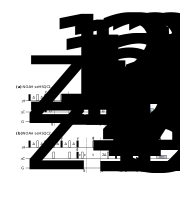
\includegraphics[]{pp/sehsqc/all_edited.png}%
    {\phantomsubcaption\label{fig:sehsqc_edited_1}}%
    {\phantomsubcaption\label{fig:sehsqc_edited_2}}%
    \caption[Multiplicity-edited NOAH seHSQC modules]{
        Multiplicity-edited NOAH seHSQC modules.
        \textbf{(\subref*{fig:sehsqc_edited_1})} Edited seHSQC1.
        \textbf{(\subref*{fig:sehsqc_edited_2})} Edited seHSQC2.
    }
    \label{fig:sehsqc_edited}
\end{figure}

\begin{figure}[!ht]
    \centering
    \includegraphics[]{noah/sehsqc_comp_edited.png}%
    {\phantomsubcaption\label{fig:noah_sehsqc_comp_edited_crk}}%
    {\phantomsubcaption\label{fig:noah_sehsqc_comp_edited_1}}%
    {\phantomsubcaption\label{fig:noah_sehsqc_comp_edited_2}}%
    \caption[Sensitivity comparisons for multiplicity-edited seHSQC]{
        Sensitivity comparisons for multiplicity-edited seHSQC in \noah{Sp,Cc} supersequences.
        The delay $\Delta'$ was set to $1 / (8 \cdot \oneJ{CH})$.
        \textbf{(\subref*{fig:noah_sehsqc_comp_edited_crk})} Using the edited CRK seHSQC.
        \textbf{(\subref*{fig:noah_sehsqc_comp_edited_1})} Using the edited seHSQC1 module.
        \textbf{(\subref*{fig:noah_sehsqc_comp_edited_2})} Using the edited seHSQC2 module.
        \datacode{7A-201115}
    }
    \label{fig:noah_sehsqc_comp_edited}
\end{figure}

The inclusion of editing does not make a substantial difference in the sensitivity comparisons (\cref{fig:noah_sehsqc_comp_edited}).
However, it is interesting to note that the edited seHSQC2 in fact performs \textit{better} than the edited HSQC in terms of preserving bulk magnetisation, as evidenced by the COSY intensities in \cref{fig:noah_sehsqc_comp_edited_2} which are greater than unity.
This can be explained by the fact that in the editing period of the HSQC experiment (and seHSQC1), the bulk magnetisation is placed in the transverse plane.
The evolution of homonuclear couplings will thus lead to a small loss in the amount of \magnnot{C} magnetisation preserved.
In the seHSQC2 sequence, the bulk magnetisation is longitudinal during the editing period, so does not evolve under $J_{\ch{HH}}$.


\subsubsection{Choice of $\symbf{\Delta'}$}

As discussed previously, there are several possible values for the delay $\Delta'$.
I also specifically investigated the possibility of setting $\Delta' = 1 / (4 \cdot \oneJ{CH})$; the corresponding sensitivity comparisons are shown in \cref{fig:noah_sehsqc_1over4j}.

\begin{figure}[!ht]
    \centering
    \includegraphics[]{noah/sehsqc_1over4j.png}%
    {\phantomsubcaption\label{fig:noah_sehsqc_1over4j_crk}}%
    {\phantomsubcaption\label{fig:noah_sehsqc_1over4j_1}}%
    {\phantomsubcaption\label{fig:noah_sehsqc_1over4j_2}}%
    \caption[Sensitivity comparisons for seHSQC with $\Delta' = 1 / (4 \cdot \oneJ{CH})$]{
        Sensitivity comparisons with $\Delta'$ set to $1 / (4 \cdot \oneJ{CH})$.
        Multiplicity editing was not used.
        \textbf{(\subref*{fig:noah_sehsqc_1over4j_crk})} Using the CRK seHSQC.
        \textbf{(\subref*{fig:noah_sehsqc_1over4j_1})} Using the seHSQC1 module.
        \textbf{(\subref*{fig:noah_sehsqc_1over4j_2})} Using the seHSQC2 module.
        \datacode{7A-201115}
    }
    \label{fig:noah_sehsqc_1over4j}
\end{figure}

As can be seen, the sensitivity boosts obtained for \ch{CH} groups are higher than in the corresponding spectra with $\Delta' = 1 / (8 \cdot \oneJ{CH})$ (\cref{fig:noah_sehsqc_comp}).
However, there is also a small sensitivity \textit{loss} for \ch{CH2} and \ch{CH3} groups as compared to the original HSQC: this is consistent with previous studies\autocite{Schleucher1994JBNMR}.
For \ch{CH3} groups, which typically have large intensities in HSQC-type spectra, this is unlikely to be of any consequence; however, for diastereotopic \ch{CH2} groups this sensitivity loss may not be desirable.

It is interesting to note that the performance of the seHSQC1 module is much closer to that of the seHSQC2 here.
The fact that seHSQC1 performs worse with the reduced value of $\Delta' = 1 / (8 \cdot \oneJ{CH})$ suggests that there are some inefficiencies in this section of the pulse sequence; however, there is no immediate explanation for this in the product operators (the relevant terms in the seHSQC1 are entirely similar to that in the CRK, save for a minus sign).

The conclusions drawn are entirely similar when multiplicity editing is enabled (\cref{fig:noah_sehsqc_1over4j_edited}), so will not be further discussed.

\begin{figure}[!ht]
    \centering
    \includegraphics[]{noah/sehsqc_1over4j_edited.png}%
    {\phantomsubcaption\label{fig:noah_sehsqc_1over4j_edited_crk}}%
    {\phantomsubcaption\label{fig:noah_sehsqc_1over4j_edited_1}}%
    {\phantomsubcaption\label{fig:noah_sehsqc_1over4j_edited_2}}%
    \caption[Sensitivity comparisons for edited seHSQC with $\Delta' = 1 / (4 \cdot \oneJ{CH})$]{
        Sensitivity comparisons with $\Delta'$ set to $1 / (4 \cdot \oneJ{CH})$ and with multiplicity editing.
        \textbf{(\subref*{fig:noah_sehsqc_1over4j_edited_crk})} Using the edited CRK seHSQC.
        \textbf{(\subref*{fig:noah_sehsqc_1over4j_edited_1})} Using the edited seHSQC1 module.
        \textbf{(\subref*{fig:noah_sehsqc_1over4j_edited_2})} Using the edited seHSQC2 module.
        \datacode{7A-201115}
    }
    \label{fig:noah_sehsqc_1over4j_edited}
\end{figure}




\subsubsection{Optimal control for seHSQC1}

One unresolved question is why the seHSQC1 module has a lower sensitivity than the seHSQC2, despite being shorter and containing fewer \ang{180} pulses.
There is also nothing in the product operator analysis to explain why this should be the case.
One remaining possibility is the presence of some non-ideality in the pulses themselves, and the composite \proton{} pulse is an obvious candidate for investigation.%
\footnote{The concept of a \textit{composite pulse}\autocite{Levitt1986PNMRS} is usually associated with greater efficiency / uniformity, but here I have used the term to loosely refer to a consecutive series of pulses.}

In order to investigate the extent to which this was responsible, I sought to use optimal control theory to develop a \textit{universal rotation pulse} (URP) which could replace this composite pulse.
Such a pulse must accomplish the transformations shown in \cref{eq:sehsqc1_dp}, namely $I_z \to I_y\/$ and $I_y \to I_x$.%
\footnote{The effect of this pulse on $x$-magnetisation is not important for the seHSQC1, but is in fact fully determined by these two constraints: $UI_x\adj{U} = -\mi U(I_yI_z - I_zI_y)\adj{U} = -\mi(UI_y\adj{U}UI_z\adj{U} - UI_z\adj{U}UI_y\adj{U}) = -\mi(I_xI_y - I_yI_x) = I_z$.
This reveals a geometric interpretation of this pulse element: it is actually a \ang{120} rotation about the vector $(1, 1, 1)$, which interchanges the three Cartesian axes; it is closely related to the $C_3$ symmetry operation in the octahedral point group.}
This optimisation was performed using an interior-point algorithm (the default in Matlab \texttt{fmincon}) and the ESCALADE method\autocite{Foroozandeh2021A} for the calculation of analytic derivatives.
Pulse fidelity was calculated as an average over 51 \proton{} spins, evenly distributed across a frequency range of \qty{11}{\kHz} (corresponding to \qty{15.7}{\ppm} at \qty{700}{\MHz}); the duration of the pulse was fixed at \qty{200}{\us}, and 200 pulse points were used.
The maximum $B_1$ allowed was \qty{15}{\kHz}; the optimisation was run with a 10\% variation in $B_1$ to minimise the effects of inhomogeneity.

The \carbon{} \ang{90} pulse which is simultaneously applied during the pulse sequence was not optimised together with this.
Since the \proton{} URP has a longer duration than this, the sequence must be modified slightly (\cref{fig:sehsqc1_urp}).
In particular, the delays $\alpha$ and $\beta$ must be chosen in order to satisfy the relations $2\varepsilon = \alpha + \beta$ (to ensure \magnnot{C} magnetisation is refocused), and $\alpha = \beta + \tau$ (to ensure that for \magn{C} magnetisation, the \carbon{} chemical shift evolves for a total duration of $t_1$).

\begin{figure}[!ht]
    \centering
    
\includegraphics[]{pp/sehsqc/1urp.png}%
    \caption[seHSQC1 pulse sequence with \proton{} URP]{
        seHSQC1 pulse sequence using a \proton{} URP in place of the double-\ang{90} composite pulse.
        $\tau$ is the difference in duration between the URP and the \carbon{} \ang{90} hard pulse.
        Delays are set as: $\alpha = \varepsilon + \tau/2$; $\beta = \varepsilon - \tau/2$.
    }
    \label{fig:sehsqc1_urp}
\end{figure}

\begin{figure}[!ht]
    \centering
    \includegraphics[]{noah/spv1_urp_magn.png}%
    {\phantomsubcaption\label{fig:spv1_urp_magn_z_x}}%
    {\phantomsubcaption\label{fig:spv1_urp_magn_z_y}}%
    {\phantomsubcaption\label{fig:spv1_urp_magn_z_z}}%
    {\phantomsubcaption\label{fig:spv1_urp_magn_z_xy}}%
    {\phantomsubcaption\label{fig:spv1_urp_magn_z_phase}}%
    {\phantomsubcaption\label{fig:spv1_urp_magn_y_x}}%
    {\phantomsubcaption\label{fig:spv1_urp_magn_y_y}}%
    {\phantomsubcaption\label{fig:spv1_urp_magn_y_z}}%
    {\phantomsubcaption\label{fig:spv1_urp_magn_y_xy}}%
    {\phantomsubcaption\label{fig:spv1_urp_magn_y_phase}}%
    \caption[Simulated performance of URP used for seHSQC1 module]{
        Simulated performance of URP used for seHSQC1 module on $z$- and $y$-magnetisation. The pulse fidelity was 99.99\%.
        \textbf{(\subref*{fig:spv1_urp_magn_z_x})--(\subref*{fig:spv1_urp_magn_z_phase})} Using $z$-magnetisation as input: the plots respectively show the amount of $x$-magnetisation, $y$-magnetisation, $z$-magnetisation, transverse magnetisation ($M_{xy} = \sqrt{M_x^2 + M_y^2}$), and the phase of the transverse magnetisation generated, as a function of offset frequency.
        \textbf{(\subref*{fig:spv1_urp_magn_y_x})--(\subref*{fig:spv1_urp_magn_y_phase})} The same, but using $y$-magnetisation as input.
    }
    \label{fig:spv1_urp_magn}
\end{figure}

This optimisation process yielded a pulse with 99.99\% fidelity: the (theoretical) performance of this pulse on $z$- and $y$-magnetisation is shown in \cref{fig:spv1_urp_magn}.
However, when tested in the actual seHSQC1 experiment, this failed to yield any substantial difference compared to the original double \ang{90} pulse (\cref{fig:sehsqc1_urp_sens_1dp,fig:sehsqc1_urp_sens_1urp}).
Importantly, the performance still falls below that of the seHSQC2 module (\cref{fig:sehsqc1_urp_sens_2}).
The reason for the poorer sensitivity therefore likely lies elsewhere.

\begin{figure}[htb]
    \centering
    \includegraphics[]{noah/sehsqc1_urp_sens.png}%
    {\phantomsubcaption\label{fig:sehsqc1_urp_sens_1dp}}%
    {\phantomsubcaption\label{fig:sehsqc1_urp_sens_1urp}}%
    {\phantomsubcaption\label{fig:sehsqc1_urp_sens_2}}%
    \caption[Sensitivity comparison of seHSQC1 module with URP]{
        Sensitivity comparisons using the seHSQC1 URP.
        $\Delta'$ was set to $1 / (8 \cdot \oneJ{CH})$; no multiplicity editing was used.
        \textbf{(\subref*{fig:sehsqc1_urp_sens_1dp})} Original seHSQC1 module with double \proton{} \ang{90} pulse.
        (Note that different datasets were used for this figure and \cref{fig:noah_sehsqc_comp}, so the numbers are very slightly different.)
        \textbf{(\subref*{fig:sehsqc1_urp_sens_1urp})} seHSQC1 using the optimised URP shown in \cref{fig:spv1_urp_magn}.
        \textbf{(\subref*{fig:sehsqc1_urp_sens_2})} seHSQC2 module for comparison.
        \datacode{7A-220110}
    }
    \label{fig:sehsqc1_urp_sens}
\end{figure}


\subsubsection{BIG-BIRD versus ZIP}

The final point in this section pertains to the implementation of the seHSQC2 module.
As it stands, the isotope-specific rotation element placed at the start of the module is the ZIP element: its role is to effect \ang{90} rotations with different phases on the \magn{C} and \magnnot{C} magnetisation pools.
However, such pulse sequence elements have been known for a long time: these include TANGO\autocite{Wimperis1984JMR}, BANGO\autocite{Sorensen1994BMR}, BIRD\autocite{Garbow1982CPL,Uhrin1993JMRSA,Kaltschnee2014CC}, BIG-BIRD\autocite{Briand1997JMR}, and TIG-BIRD\autocite{Briand1998JMR}.
In particular, the BIG-BIRD element, which allows for independent excitation of \magn{C} and \magnnot{C} magnetisation with arbitrary flip angles and phases, can be designed to accomplish the same overall effect as the ZIP element.
For the seHSQC2 without multiplicity editing, the relevant BIG-BIRD sequence is
\begin{equation}
    \label{eq:big_bird_unedited}
    45\rlap{\unit{\degree}}_{\ang{45}}(\proton{})\text{--}2\Delta\text{--}\ang{180}(\proton{},\carbon{})\text{--}2\Delta\text{--}45\rlap{\unit{\degree}}_{\ang{225}}(\proton{}),
\end{equation}
where $\beta_\phi$ represents a hard pulse with flip angle $\beta$ and phase $\phi$.
For the edited seHSQC2, the phases must be altered slightly:
\begin{equation}
    \label{eq:big_bird_edited}
    45\rlap{\unit{\degree}}_{\ang{315}}(\proton{})\text{--}2\Delta\text{--}\ang{180}(\proton{},\carbon{})\text{--}2\Delta\text{--}45\rlap{\unit{\degree}}_{\ang{135}}(\proton{}).
\end{equation}
\Cref{fig:noah_sehsqc_bigbird} provides sensitivity comparisons between the BIG-BIRD and ZIP versions of the seHSQC2.
The fact that similar numbers were achieved with both elements indicates that the BIG-BIRD element is (largely) effecting the desired rotations on the different magnetisation pools.
However, in all respects, the performance of the BIG-BIRD sequence was not as good as the ZIP version: both the seHSQC sensitivity itself, as well as the sensitivity of the later CLIP-COSY, were slightly decreased when the BIG-BIRD element was used.
This is true regardless of whether multiplicity editing was used.

\begin{figure}[!ht]
    \centering
    \includegraphics[]{noah/sehsqc_bigbird.png}%
    {\phantomsubcaption\label{fig:noah_sehsqc_bigbird_bb_noed}}%
    {\phantomsubcaption\label{fig:noah_sehsqc_bigbird_zip_noed}}%
    {\phantomsubcaption\label{fig:noah_sehsqc_bigbird_bb_ed}}%
    {\phantomsubcaption\label{fig:noah_sehsqc_bigbird_zip_ed}}%
    \caption[Comparison of BIG-BIRD and ZIP pulse elements in seHSQC2 module]{
        Sensitivity comparisons of BIG-BIRD and ZIP pulse elements in seHSQC2 module.
        The reference dataset being compared against is still the \noah{S,Cc} (but with editing in (\subref*{fig:noah_sehsqc_bigbird_bb_ed}) and (\subref*{fig:noah_sehsqc_bigbird_zip_ed}).
        The delay $\Delta'$ was set to $1 / (8 \cdot \oneJ{CH})$.
        \textbf{(\subref*{fig:noah_sehsqc_bigbird_bb_noed})} Unedited seHSQC2 using BIG-BIRD.
        \textbf{(\subref*{fig:noah_sehsqc_bigbird_zip_noed})} Unedited seHSQC2 using ZIP.
        \textbf{(\subref*{fig:noah_sehsqc_bigbird_bb_ed})} Edited seHSQC2 using BIG-BIRD.
        \textbf{(\subref*{fig:noah_sehsqc_bigbird_zip_ed})} Edited seHSQC2 using ZIP.
        \datacode{7A-201115}
    }
    \label{fig:noah_sehsqc_bigbird}
\end{figure}

\subsection{\texorpdfstring{\nitrogen{}}{15N} HMQC}
\label{subsec:noah__hmqc}

In \cref{subsec:noah__sehsqc_n}, I will discuss how the sensitivity-enhanced HSQC modules developed above may be adapted into \proton{}--\nitrogen{} experiments.
However, before that, I make a slight detour to cover the \nitrogen{} HMQC experiment, which (up until my DPhil) was the experiment of choice for detecting one-bond \proton{}--\nitrogen{} correlations.

\begin{figure}[htb]
    \centering
    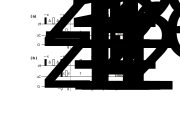
\includegraphics[draft=false]{pp/hmqc/all.png}%
    {\phantomsubcaption\label{fig:noah_hmqc_2grad}}%
    {\phantomsubcaption\label{fig:noah_hmqc_4grad}}%
    \caption[NOAH HMQC pulse sequences]{
        \textbf{(\subref{fig:noah_hmqc_2grad})} With two encoding gradients around $t_1$.
        \textbf{(\subref{fig:noah_hmqc_4grad})} With four encoding gradients around $t_1$.
        Phase cycling is performed with $\phi_1 = (x, -x)$, $\phi_2 = (x, x, -x, -x)$, and $\phi_\text{rec} = (x, -x, -x, x)$.
        The delay $\Delta$ is set to $1 / (4 \cdot \oneJ{NH})$.
        Gradient amplitudes are: $g_1 = 80\%$; $g_2 = \pm 32.4\%$; $g_2' = g_2/2$.
    }
    \label{fig:noah_hmqc}
\end{figure}

The HMQC module is based on the ASAP-HMQC reported by Kup{\v{c}}e and Freeman\autocite{Kupce2007MRC}, which used a symmetric gradient scheme similar to that in the seHSQC modules previously described (\cref{fig:noah_hmqc_2grad}).
However, in the NOAH module\autocite{Kupce2017ACIE}, bipolar gradient pulse pairs were placed before and after $t_1$ (\cref{fig:noah_hmqc_4grad}).
This was likely implemented in order to allow the final gradient, $g_2$, to have as large an amplitude as possible.
In heteronuclear experiments, this final gradient is particularly important for dephasing bulk magnetisation which is transverse just prior to detection (due to pulse imperfections or relaxation).
If this gradient is too weak, this unwanted magnetisation will be incompletely dephased, leading to artefacts in the resulting spectrum.

Strategies to maximise this gradient amplitude are particularly crucial in \proton{}--\nitrogen{} experiments (as compared to \proton{}--\carbon{} experiments) for two reasons.
Firstly, the natural abundance of \nitrogen{} (0.36\%) is even smaller than \carbon{} (1.1\%), meaning that better suppression must be achieved in order for the artefacts to not obscure the signal.
Secondly, the gyromagnetic ratio of \nitrogen{} is also smaller: thus, since $g_2/g_1 \propto \gammaN/\gammaH$, an unmodified pulse sequence will naturally have a smaller $g_2$.

In this respect, the four-gradient scheme in \cref{fig:noah_hmqc_4grad} is superior to the two-gradient scheme, because the gradient $g_2$ will have an amplitude of $4\gammaN g_1/\gammaH$.
However, when used in a NOAH supersequence, this leads to wing artefacts in downstream modules, since bulk \magnnot{N} magnetisation effectively does not experience any coherence order selection during $t_1$.
This motivates a return to the two-gradient scheme of \cref{fig:noah_hmqc_2grad}.
To compensate for the fact that the decoding gradient $g_2'$ has half of the amplitude of $g_2$, all CTP gradients were instead \textit{lengthened} from their usual duration of \qty{1}{\ms} to \qty{2.5}{\ms}.
This ensures that any stray transverse bulk magnetisation at the end of the HMQC module is effectively dephased.

The HMQC spectra thus obtained are shown in \cref{fig:hmqc_grad_spec}.

\begin{figure}[!ht]
    \centering
    \includegraphics[draft=false]{noah/hmqc_grad.png}%
    {\phantomsubcaption\label{fig:hmqc_grad_spec_2grad_1ms_hmqc}}%
    {\phantomsubcaption\label{fig:hmqc_grad_spec_2grad_1ms_hmqcp}}%
    {\phantomsubcaption\label{fig:hmqc_grad_spec_2grad_1ms_cosy}}%
    {\phantomsubcaption\label{fig:hmqc_grad_spec_4grad_1ms_hmqc}}%
    {\phantomsubcaption\label{fig:hmqc_grad_spec_4grad_1ms_hmqcp}}%
    {\phantomsubcaption\label{fig:hmqc_grad_spec_4grad_1ms_cosy}}%
    {\phantomsubcaption\label{fig:hmqc_grad_spec_2grad_2p5ms_hmqc}}%
    {\phantomsubcaption\label{fig:hmqc_grad_spec_2grad_2p5ms_hmqcp}}%
    {\phantomsubcaption\label{fig:hmqc_grad_spec_2grad_2p5ms_cosy}}%
    \caption[Comparison of \noah{M,Sp,Cc} modules with different HMQC gradient schemes]{
        Comparison of HMQC and CLIP-COSY spectra obtained from \noah{M,Sp,Cc} supersequences, acquired using different HMQC gradient schemes.
        In the first row, the HMQC spectrum itself is shown.
        In the second row, the positive projection of the HMQC spectrum onto the $f_2$ axis is shown; the numbers indicate peak intensities with respect to the reference dataset (the left column).
        In the third row, (an inset of) the CLIP-COSY spectrum is shown.
        \textbf{(\subref{fig:hmqc_grad_spec_2grad_1ms_hmqc})--(\subref{fig:hmqc_grad_spec_2grad_1ms_cosy})} Using the two-gradient scheme of \cref{fig:noah_hmqc_2grad}, with \qty{1}{ms} gradients.
        \textbf{(\subref{fig:hmqc_grad_spec_4grad_1ms_hmqc})--(\subref{fig:hmqc_grad_spec_4grad_1ms_cosy})} Using the four-gradient scheme of \cref{fig:noah_hmqc_4grad}, with \qty{1}{ms} gradients.
        \textbf{(\subref{fig:hmqc_grad_spec_2grad_2p5ms_hmqc})--(\subref{fig:hmqc_grad_spec_2grad_2p5ms_cosy})} Using the two-gradient scheme of \cref{fig:noah_hmqc_2grad}, with \qty{2.5}{ms} gradients.
    }
    \label{fig:hmqc_grad_spec}
\end{figure}

\subsection{\texorpdfstring{\nitrogen{}}{15N} sensitivity-enhanced HSQC}
\label{subsec:noah__sehsqc_n}

I now move on to the \nitrogen{} seHSQC experiment, which (for small molecules) is an improvement on the HMQC experiment for two reasons: firstly, the PEP transfer grants additional sensitivity (and can be optimised for \ch{NH} groups); and secondly, splittings due to $\nJ{HH}$ are not observed in the indirect dimension.


\subsubsection{seHSQC sensitivity}



\subsubsection{Sensitivity of later modules}



\subsubsection{$k$-Scaling and linear prediction}


\subsection{HSQC-TOCSY}
\label{subsec:noah__hsqctocsy}

Having completed our survey of \nitrogen{} modules, we now return to \carbon{} modules: in particular, I was particularly interested in how \textit{two} (or more) modules drawing on \magn{C} magnetisation could be combined in the same supersequence.
Of course, this can be crudely accomplished by simply concatenating two modules which consume all \magn{C} magnetisation: the second of these modules will have greatly reduced sensitivity.
This is acceptable if the second module has a far greater intrinsic sensitivity, but this is not often the case with heteronuclear experiments: thus, a method of \textit{balancing} the sensitivities of the two modules is desirable.
Equivalently, we would like a way to \textit{partition} the magnetisation pool between multiple different modules as we see fit.


\subsubsection{Two HSQC modules}

The strategy used here is in fact a feature of the ASAP-HSQC experiment\autocite{SchulzeSunninghausen2014JACS,SchulzeSunninghausen2017JMR}, previously described in \cref{subsec:poise__asaphsqc}.
In this experiment (which also doubles up as the NOAH HSQC module), the INEPT delay $\DeltaE$ can be changed from its usual value of $1 / (4J)$ (where $J$ is short for $\oneJ{CH}$).
After the \ang{90}($I$)--$\DeltaE$--\ang{180}($I,S$)--$\DeltaE$ INEPT block, the relevant product operators are
\begin{equation}
    \label{eq:inept_changed}
    \cos(2\pi J\DeltaE) I_y - \sin(2\pi J\DeltaE) 2I_xS_z.
\end{equation}
In a `normal' INEPT block, the choice of $\DeltaE = 1/(4J)$ makes the cosine term vanish, leaving us with only the term $-2I_xS_z$.
Since this term is subsequently transferred to spin $S\/$ and labelled in $t_1$, this corresponds to \textit{complete} excitation of \magn{C} magnetisation.

However, if we choose $\DeltaE < 1/(4J)$, then the first $I_y$ term can be `stored' as unexcited \magn{C} magnetisation;
if the remainder of the sequence returns \textit{this} to the $+z$ state, then this portion can be used in a second experiment.
Indeed, this is what happens in the ASAP-HSQC experiment (i.e.\ NOAH HSQC module).
Thus, we could simply construct a \noah{S,S,C} experiment in which the first HSQC module has a suitably modified value of $\DeltaE$: this would achieve the stated aim of partitioning \magn{C} magnetisation between two different modules.
Specifically, in order to excite a fraction $f\/$ of \magn{C} magnetisation (and store the remaining $(1 - f)$ for the next module), we require that
\begin{equation}
    \label{eq:ssc_inept_delay}
    \DeltaE = \frac{2\Delta \arcsin f}{\pi}
\end{equation}
where $\Delta$ is the usual value of $1/(4J)$.
The resulting spectra, obtained by setting $f = 0.8$, are shown in \cref{fig:sscc_example}.


\begin{figure}[!ht]
    \centering
    \includegraphics[draft=false]{noah/sscc_example.png}%
    {\phantomsubcaption\label{fig:sscc_example_s1}}%
    {\phantomsubcaption\label{fig:sscc_example_s2}}%
    {\phantomsubcaption\label{fig:sscc_example_cc}}%
    \caption[Spectra from \noah{S,S,Cc} supersequence]{
        Spectra from a \noah{S,S,Cc} supersequence, where the INEPT delay of the first HSQC module was modified to only excite a fraction $f = 0.7$ of \magn{C} magnetisation.
        \textbf{(\subref*{fig:sscc_example_s1})} First HSQC.
        \textbf{(\subref*{fig:sscc_example_s2})} Second HSQC.
        \textbf{(\subref*{fig:sscc_example_cc})} CLIP-COSY.
        \datacode{7A-201010}
    }
    \label{fig:sscc_example}
\end{figure}

In \cref{fig:sscc_improvements_base}, the intensities of these spectra are compared against the HSQC and CLIP-COSY in a \noah{S,Cc} supersequence.
As expected, the first HSQC has 80\% of its sensitivity.
However, the second HSQC spectrum has around 65\% of this `base' sensitivity, despite only nominally having 20\% of the \magn{C} magnetisation to work with.
This is largely due to \magn{C} magnetisation which recovers during the FID of the first HSQC.
Since both HSQC modules do not perfectly preserve \magnnot{C} magnetisation, the CLIP-COSY experiences a very small sensitivity loss (compared to a \noah{S,Cc} supersequence where only one HSQC module is used, which in turn is slightly less sensitive than a standalone CLIP-COSY).

\begin{figure}[!ht]
    \centering
    \includegraphics[draft=false]{noah/sscc_improvements.png}%
    {\phantomsubcaption\label{fig:sscc_improvements_base}}%
    {\phantomsubcaption\label{fig:sscc_improvements_sehsqc}}%
    {\phantomsubcaption\label{fig:sscc_improvements_dipsi}}%
    {\phantomsubcaption\label{fig:sscc_improvements_mfa}}%
    \caption[Sensitivity comparisons for \noah{S,S,Cc} and \noah{S,Sp,Cc} supersequences]{
        Comparisons of HSQC and CLIP-COSY sensitivities of \noah{S,S,Cc} and \noah*{S,Sp,Cc} supersequences.
        The fraction of \magn{C} magnetisation excited in the first module, $f$, is set to $0.8$.
        Peak intensities are normalised against the HSQC and CLIP-COSY experiments in a \noah{S,Cc} supersequence.
        \textbf{(\subref*{fig:sscc_improvements_base})} \noah{S,S,Cc} (the same spectra as shown in \cref{fig:sscc_example}).
        \textbf{(\subref*{fig:sscc_improvements_sehsqc})} \noah{S,Sp,Cc}.
        \textbf{(\subref*{fig:sscc_improvements_dipsi})} \noah{S,S,Cc} with \qty{35}{\ms} DIPSI-2 mixing after the first HSQC module.
        \textbf{(\subref*{fig:sscc_improvements_mfa})} A \noah{S,S,Cc} supersequence, but using the seHSQC-splitting implementation of Nolis et al.\autocite{Nolis2019CPC} (as opposed to the ASAP-HSQC module) for the double HSQC.
    }
    \label{fig:sscc_improvements}
\end{figure}

The sensitivity of the second HSQC module can be further improved by simply using the seHSQC module (specifically, the seHSQC2) in place of it.
The effects of this are shown in \cref{fig:sscc_improvements_sehsqc}: sensitivity improvements are obtained in that module itself (although they are not uniform as they depend on multiplicity), and the CLIP-COSY sensitivity is decreased slightly due to poorer \magnnot{C} preservation.
These are entirely in line with the previous discussion in \cref{subsec:noah__sehsqc_c}.

It is also possible to include a period of isotropic mixing between the two HSQC modules: here, the DIPSI-2 sequence\autocite{Shaka1988JMR} was chosen.
Since the \magn{C} magnetisation pool has been (partially) depleted, and the \magnnot{C} magnetisation pool is (almost) full, this should in theory lead to transfer of polarisation from the \magnnot{C} pool to \magn{C}.
However, when tested, this was not found to have a beneficial impact on the supersequence sensitivity (\cref{fig:sscc_improvements_dipsi}): in fact, 
One caveat is that this leads to slightly uneven intensities: since DIPSI transfers magnetisation through scalar couplings, peaks corresponding to protons with fewer coupling partners experience smaller gains in intensity.

\todo{Pulse sequence with prod ops??}

\todo{Multiplicity editing --- not properly implemented in GENESIS?!}


On its own, the acquisition of two HSQC spectra---as has so far been shown---is not particularly interesting.
However, it is possible to differentiate the two HSQC signals and thereby extract more information.
For example, one spectrum may be run without decoupling in order to measure one-bond coupling constants\autocite{Enthart2008JMR,Nolis2019CPC}; or the indirect-dimension spectral width of one of the HSQC spectra can be changed in order to make use of spectral aliasing techniques\autocite{Nolis2019JMR,Jeannerat2011eMR}.
The pulse sequence itself may also be modified: for example, the addition of an isotropic mixing block to the first HSQC yields a HSQC-TOCSY + HSQC combination\autocite{Nolis2019CPC}, which I now discuss.


\subsubsection{HSQC-TOCSY}

The addition of DIPSI mixing
This in fact leads to the ASAP-HSQC-TOCSY experiment, also previously reported by Luy and coworkers\autocite{Becker2019JMR}.


\subsection{HSQC-COSY}
\label{subsec:noah__hsqc_cosy}

Blah.

\subsection{2DJ and PSYCHE}
\label{subsec:noah__2djpsyche}

So far, I have exclusively used the CLIP-COSY as the final homonuclear module in NOAH supersequences.
In general, since homonuclear modules are placed at the end of supersequences, there is rarely any need to adapt them for NOAH supersequences, as they do not need to preserve any magnetisation.
One exception to this is the family of 2DJ and pseudo-2D pure shift experiments (here typified by PSYCHE), where the spectral width in the indirect dimension is extremely small, on the order of \qty{50}{\Hz}.
In such cases, the number of $t_1$ increments required is far smaller than for a typical 2D experiment.
Since---by default---each module in a NOAH supersequence is acquired with the same number of increments, directly concatenating such modules to the end of a supersequence would therefore prove suboptimal.

However, as described previously in \cref{subsec:noah__hmqc,subsec:noah__sehsqc_n}, it is possible to reduce the number of $t_1$ increments for a particular module, and in exchange, increase the number of scans recorded for that module.
In the context of \nitrogen{} modules, this was a `special' procedure referred to as $k$-scaling; however, for these homonuclear modules, it is natural and necessary.
One difference in the implementation is that, instead of specifying a value $k$ by which \texttt{TD1} is scaled down and \texttt{NS} scaled up, the user is allowed to directly specify the number of $t_1$ increments as an integer (\texttt{CNST37} in TopSpin).
This value must be a divisor of the \textit{normal} number of $t_1$ increments for all other modules (or equivalently, in the context of \nitrogen{} modules, $k$ must be an integer).
The `indirect-dimension spectral width' is specified as \texttt{CNST38}: this quantity is more properly referred to as the reciprocal of the chunk size, i.e.\ $1/\Tchunk$.

\begin{figure}[!ht]
    \centering
    \includegraphics[]{noah/2dj_example.png}%
    {\phantomsubcaption\label{fig:2dj_example_spn}}%
    {\phantomsubcaption\label{fig:2dj_example_spc}}%
    {\phantomsubcaption\label{fig:2dj_example_j}}%
    \caption[Spectra from a \noah{Spn,Sp,J} supersequence]{
        Spectra obtained from a \noah{Spn,Sp,J} supersequence.
        \textbf{(\subref*{fig:2dj_example_spn})} \nitrogen{} seHSQC (256 $t_1$ increments and 2 scans per increment).
        \textbf{(\subref*{fig:2dj_example_spc})} \carbon{} seHSQC.
        \textbf{(\subref*{fig:2dj_example_j})} PSYCHE 2DJ (32 $t_1$ increments and 8 scans per increment).
        \datacode{7G-201028}
    }
    \label{fig:2dj_example}
\end{figure}

The modules thus implemented include the standard magnitude-mode 2DJ experiment, the PSYCHE 2DJ experiment\autocite{Foroozandeh2015CC}, the original 1D PSYCHE\autocite{Foroozandeh2014ACIE}, and the 1D TSE-PSYCHE\autocite{Foroozandeh2015CC}.
An example of the data thus obtained (with the PSYCHE 2DJ) is shown in \cref{fig:2dj_example}.
One particular advantage of including PSYCHE-type modules in NOAH supersequences is that sensitivity is not likely to be at a premium: this is partly because of the increased number of scans, but also partly because other 2D experiments have comparably low sensitivity (meaning that in the time needed to acquire an HSQC, for example, the PSYCHE experiment will also have sufficient sensitivity).
This allows the user to choose a relatively small flip angle (ca.\ \ang{10}) for the PSYCHE saltire pulses in order to minimise artefacts from imperfect decoupling (see also \cref{subsec:pureshift__psyche_analysis}).

\begin{figure}[!ht]
    \centering
    \includegraphics[]{noah/psyche_wrongsw1.png}%
    {\phantomsubcaption\label{fig:psyche_wrongsw1_bad_nosap}}%
    {\phantomsubcaption\label{fig:psyche_wrongsw1_bad_sap}}%
    {\phantomsubcaption\label{fig:psyche_wrongsw1_good_nosap}}%
    {\phantomsubcaption\label{fig:psyche_wrongsw1_good_sap}}%
    {\phantomsubcaption\label{fig:psyche_wrongsw1_good_nosap_25}}%
    {\phantomsubcaption\label{fig:psyche_wrongsw1_good_sap_25}}%
    \caption[Effect of automatic chunk size calculation and SAPPHIRE averaging on NOAH PSYCHE spectra]{
        A series of 1D PSYCHE spectra obtained from the \noah{Spn,Sp,P} supersequence (saltire flip angle of \ang{15}).
        \textbf{(\subref*{fig:psyche_wrongsw1_bad_nosap})} 1D PSYCHE spectrum acquired without SAPPHIRE averaging, and an incorrect chunk size which is not an integral number of complex data points. The `indirect-dimension spectral width' (more precisely, $1/\Tchunk$) is \qty{50}{\Hz}.
        \textbf{(\subref*{fig:psyche_wrongsw1_bad_sap})} 1D PSYCHE spectrum with  8-step SAPPHIRE averaging and an incorrect chunk size; this manifests as phase errors which cannot be corrected.
        \textbf{(\subref*{fig:psyche_wrongsw1_good_nosap})--(\subref*{fig:psyche_wrongsw1_good_sap})} The same as (\subref*{fig:psyche_wrongsw1_bad_nosap}) and (\subref*{fig:psyche_wrongsw1_bad_sap}), but with the chunk size automatically corrected in the pulse programme.
        \textbf{(\subref*{fig:psyche_wrongsw1_good_nosap_25})--(\subref*{fig:psyche_wrongsw1_good_sap_25})} The same as (\subref*{fig:psyche_wrongsw1_good_nosap}) and (\subref*{fig:psyche_wrongsw1_good_sap}), but with double the chunk size.
        This leads to a more striking difference between the data acquired without and with SAPPHIRE, as discussed in the original paper\autocite{Moutzouri2017CC}.
        \datacode{7C-211123}
    }
    \label{fig:psyche_wrongsw1}
\end{figure}

On top of this, for the 1D (TSE-)PSYCHE sequences, the extra transients can be used to perform SAPPHIRE averaging\autocite{Moutzouri2017CC}.
Ordinarily, the PSYCHE pulse sequence seeks to refocus J-couplings in the middle of each chunk (of duration $\Tchunk$).
This is accomplished through the \textit{prefocusing} of J-couplings in a spin echo of total duration $\Tchunk/2$.\autocite{Aguilar2010ACIE}
In the SAPPHIRE procedure, each chunk of the pure shift interferogram is instead collected several times, all while varying the exact point in time where J-coupling is perfectly refocused.
Summation of these data leads to the suppression of artefacts which arise due to the periodic J-modulation in the interferogram.
This averaging is somewhat analogous to a phase cycle, and performing an 8-step SAPPHIRE averaging procedure (for example) would often require the experiment to be lengthened beyond the duration which is truly necessary.
However, in the context of NOAH, since each chunk is acquired at least $k$ times, a $k$-step SAPPHIRE procedure can be performed `for free'.
In the GENESIS pulse programmes, this feature is enabled by default, although it can be turned off by selecting the original modules using developer mode.

A final and more prosaic implementation detail is that in the 1D pure shift modules, the chunk size $\Tchunk$ is automatically rounded to the nearest even multiple of the dwell time $\tau_{\symup{dw}}$ (\texttt{DW} in TopSpin).
This ensures that each chunk consists of an integral number of complex data points.
Although this can be set by the user manually, it is very easy to forget, especially for someone not fully acquainted with the experiment; the results can be quite different, as illustrated in \cref{fig:psyche_wrongsw1}.
When an $n$-step SAPPHIRE averaging is used, the requirement is even stricter: $\Tchunk$ must be a multiple of $2n \tau_{\symup{dw}}$.
This is also encoded in the pulse programmes.

\subsection{HMBC}
\label{subsec:noah__hmbc}

The HMBC module is one which in fact does not fit perfectly into the NOAH principle of only exciting magnetisation which is needed.
As described in \cref{subsec:noah__case_studies}, the HMBC module should only require magnetisation of protons which have long-range couplings to \carbon{}; however, it ends up exciting \textit{all} \magnnot{C} magnetisation.
This leads to sharply reduced, and also unbalanced, intensities of homonuclear modules which come later in the supersequences.

I made some early (and brief) attempts at devising a pulse sequence which sought to discriminate these two magnetisation components using a perfect echo\autocite{Parella2019MRC}.
However, this was quickly abandoned as it proved very difficult to \textit{also} retain \magn{C} magnetisation.
I do not claim here that it is impossible to come up with a pulse sequence which does this, but it is certainly not easy, and ultimately I turned my focus to improving (rather than replacing) the HMBC module.


\subsubsection{Suppression of one-bond artefacts}

One of the issues with the NOAH HMBC module was that there were an unusual amount of one-bond artefacts, which arise from \magn{C} magnetisation which is allowed to evolve during the pulse sequence.
Generally, HMBC experiments seek to suppress this through the use of a low-pass J-filter (LPJF, see also \cref{subsec:poise__hmbc}).
The NOAH HMBC module \textit{additionally} contains a $zz$-filter, which stores \magn{C} magnetisation along $+z$ before the LPJF.
Thus, in theory, one-bond artefacts should be suppressed in the NOAH HMBC to an even greater extent.

However, this expectation is not borne out: in some cases, the NOAH HMBC in fact has \textit{more intense} one-bond artefacts when compared against a standard HMBC experiment (\cref{fig:noah_hmbc_1jch_no90,fig:noah_hmbc_1jch_std_lp2}).
Even performing an optimisation of the LPJF delays, as described in \cref{subsec:poise__hmbc}, did not lead to any reduction in artefacts.
I hypothesised instead that these artefacts arose from imperfect manipulation of \magn{C} magnetisation by the $zz$-filter.%
\footnote{It would be nice to back this up with simulations, but I did not have the time to run these.}
In particular, any \textit{antiphase} magnetisation (of the form $I_xS_z$ or $I_yS_z$) generated after the $zz$-filter would be reconverted into in-phase $I_x$ or $I_y$ terms, which would not be destroyed by the LPJF.
(The LPJF works based on the assumption that there is in-phase magnetisation at the beginning of it, which is true if the excitation element is just a \proton{} \ang{90} pulse.)

Such antiphase terms can be easily removed by the addition of a \carbon{} \ang{90} pulse, which transforms them into a mixture of double- and zero-quantum terms: these are either unobservable, or can be efficiently dephased by CTP gradients.
This technique is used in the CLIP-HSQC family of experiments\autocite{Enthart2008JMR,Gyongyosi2021AC}, as well as the LPJF itself.
In this case, we simply need to add an additional \carbon{} \ang{90} pulse at the end of the $zz$-filter: this pulse is highlighted in \cref{fig:noah_sb_po_b}.
This results in a striking reduction of the one-bond artefacts, as shown in \cref{fig:noah_hmbc_1jch_90}.
The suppression accomplished with the addition of this \ang{90} pulse is superior to that in the standard HMBC (\cref{fig:noah_hmbc_1jch_std_lp2}), and is comparable to a standard HMBC with a third-order LPJF (\cref{fig:noah_hmbc_1jch_std_lp3}).
Of course, the NOAH module---which by default uses a second-order LPJF---can also be `upgraded' to use a third-order LPJF.
In GENESIS pulse programmes, this can be done using the \texttt{-DLP3} acquisition flag (although the results were not evaluated here).

\begin{figure}[!ht]
    \centering
    \includegraphics[]{noah/hmbc_1jch.png}%
    {\phantomsubcaption\label{fig:noah_hmbc_1jch_no90}}%
    {\phantomsubcaption\label{fig:noah_hmbc_1jch_90}}%
    {\phantomsubcaption\label{fig:noah_hmbc_1jch_std_lp2}}%
    {\phantomsubcaption\label{fig:noah_hmbc_1jch_std_lp3}}%
    \caption[Suppression of one-bond artefacts in NOAH HMBC spectra]{
        \textbf{(\subref*{fig:noah_hmbc_1jch_no90})} NOAH $zz$-HMBC module without the additional \ang{90} pulse.
        One-bond artefacts are highlighted in red.
        \textbf{(\subref*{fig:noah_hmbc_1jch_90})} NOAH $zz$-HMBC with the \ang{90} pulse.
        \textbf{(\subref*{fig:noah_hmbc_1jch_std_lp2})} Standard library HMBC with a second-order LPJF.
        \textbf{(\subref*{fig:noah_hmbc_1jch_std_lp3})} Standard library HMBC with a third-order LPJF.
        \datacode{7A-210916}
    }
    \label{fig:noah_hmbc_1jch}
\end{figure}


\subsubsection{Gradient selection schemes}

Another point which was investigated (but bore less fruit) was the gradient scheme used for CTP selection.
The NOAH module, as shown in \cref{fig:noah_sb_po_b}, uses a `symmetric' scheme where two gradients of equal amplitude surround the $t_1$ period: this encoding is later decoded by a third gradient just prior to acquisition.
However, other choices exist: for example, the Bruker standard library HMBC (derived from the work of Cicero et al.\autocite{Cicero2001JMR}) uses only two gradients in total, which have unequal amplitudes.

This gradient scheme cannot be directly used in a NOAH HMBC module, though.
This is because the $zz$-filter element places \magn{C} magnetisation along the $+z$ axis just before the HMBC J-evolution delay (see \cref{fig:noah_sb_po_b}).
This magnetisation later experiences the \proton{} \ang{180} pulse in the middle of $t_1$, which means that an extra \ang{180} pulse must be added at the very end of the sequence to finally return it to $+z$.
It is necessary to ensure that there is at least one gradient placed after this \ang{180} pulse to ensure proper CTP selection (in the `symmetric' scheme of \cref{fig:noah_sb_po_b}, this is fulfilled by the gradient $g_2$).

\begin{figure}[!htbp]
    \centering
    
\includegraphics[]{pp/hmbc/noah_grads.png}%
    {\phantomsubcaption\label{fig:noah_hmbc_grads_bga}}%
    {\phantomsubcaption\label{fig:noah_hmbc_grads_bgb}}%
    {\phantomsubcaption\label{fig:noah_hmbc_grads_bgc}}%
    {\phantomsubcaption\label{fig:noah_hmbc_grads_b}}%
    \caption[Alternative CTP gradient schemes investigated for NOAH HMBC]{
        Alternative CTP gradient schemes investigated for the NOAH HMBC module.
        The coherences selected for during each gradient are indicated above each gradient, using the same notation for product operators as described in the \textit{Preface}: the `upper' term (e.g.\ $+$ in $\pm$) refers to the echo experiment, and the `lower' term to the antiecho experiment.
        So, for example, $+\pm$ refers to selection of $I_+S_+$ during the echo experiment and $I_+S_-$ during the antiecho experiment.
        Gradient amplitudes are as described in the text.
        \textbf{(\subref*{fig:noah_hmbc_grads_bga})} `Asymmetric scheme A', modified from the standard library sequence to include an additional \ang{180} pulse and gradient.
        \textbf{(\subref*{fig:noah_hmbc_grads_bgb})} `Asymmetric scheme B', where the \ang{180} pulse is shifted forward to the end of $t_1$.
        \textbf{(\subref*{fig:noah_hmbc_grads_bgc})} `Asymmetric scheme C', which modifies the $zz$-filter instead of using an extra \ang{180} pulse.
        \textbf{(\subref*{fig:noah_hmbc_grads_b})} The original `symmetric' scheme (the same as in \cref{fig:noah_sb_po_b}), placed here for convenience.
    }
    \label{fig:noah_hmbc_grads}
\end{figure}

Using this knowledge, it is possible to construct several `asymmetric' gradient schemes:
\begin{enumerate}
    \item `Scheme A' (\cref{fig:noah_hmbc_grads_bga}) is modified from the Bruker standard library to include a \ang{180} pulse and gradient at the end.
        The presence of an additional gradient means that there is a free parameter, here denoted as $\alpha$, which can be used to control the relative amplitudes of these three CTP gradients.
        The gradient amplitudes are chosen as follows:
        \begin{align}
            &\text{echo:}     & g_1 &= gc_1 & g_2 &= g    & g_3 &= gc_2 \label{eq:noah_hmbc_grads_bga_echo} \\
            &\text{antiecho:} & g_1 &= g    & g_2 &= gc_1 & g_3 &= gc_2 \label{eq:noah_hmbc_grads_bga_antiecho}
        \end{align}
        where $c_1 = -\alpha(\gammaH - \gammaC)/(\gammaH + \gammaC)$ and $c_2 = (1 - \alpha) (\gammaH - \gammaC)/\gammaH$.
        In principle $g$ is also a free parameter; for maximum suppression of artefacts I chose a relatively large value of 80\%.
    \item In `Scheme B' (\cref{fig:noah_hmbc_grads_bgb}), the \ang{180} pulse is shifted to immediately after $t_1$, before any of the CTP gradients have been applied. This means that there is no need for a third gradient, and the CTP gradient amplitudes can be directly taken from the standard library sequence:
        \begin{align}
            &\text{echo:}     & g_1 &= g  & g_2 &= gc \label{eq:noah_hmbc_grads_bgb_echo} \\
            &\text{antiecho:} & g_1 &= gc & g_2 &= g \label{eq:noah_hmbc_grads_bgb_antiecho}
        \end{align}
        where $c = -(\gammaH - \gammaC)/(\gammaH + \gammaC)$ and $g = 80\%$.
    \item `Scheme C' (\cref{fig:noah_hmbc_grads_bgc}) simply does not add a \ang{180} pulse, but instead modifies the phases of the $zz$-filter in order to place \magn{C} magnetisation along the $-z$ axis during the HMBC J-evolution delay.
        Here, the gradient amplitudes are the same as those in the standard library sequence as well as in scheme B.
\end{enumerate}

It is of interest to note two limiting cases of scheme A: when $\alpha = (\gammaH + \gammaC)/(\gammaH - \gammaC) \approx 1.67$, we have that $g_1 : g_2 : g_3 = 1 : -1 : \pm 2\gammaC/\gammaH$, which mimics the original `symmetric' scheme (\cref{fig:noah_hmbc_grads_b}); and when $\alpha = 1$, we have that $g_3 = 0$, i.e.\ a return to the two-gradient tactic of schemes B and C.
In the tests which follow, I ran scheme A with $\alpha = 1.67$, $\alpha = 0.6$, and $\alpha = 0.3$.

\begin{figure}[htb]
    \centering
    \includegraphics[]{noah/hmbc_grad_sens.png}%
    \caption[Comparison of relative sensitivities of HMBC gradient schemes]{
        Sensitivities of various asymmetric HMBC gradient schemes, as compared to the symmetric scheme in \cref{fig:noah_sb_po_b}.
        Each dot indicates one crosspeak in the HMBC spectrum; the numbers in parentheses are the average over all peaks.
        \datacode{7A-211226}
    }
    \label{fig:hmbc_grad_sens}
\end{figure}

All of the different HMBC versions above, plus the original `symmetric' scheme in \cref{fig:noah_sb_po_b}, were tested in the context of a \noah{B,S} supersequence using the andrographolide sample (\cref{fig:hmbc_grad_sens}).
Since the HMBC module is the first module in this supersequence, the values here are an accurate reflection of their intrinsic sensitivities.
As can be seen, there is not much at all which separates the different versions (outliers with $>2\times$ `sensitivity improvements' can be attributed to different J-modulation in the multiplet).
The most sensitive of these is asymmetric scheme C, which may be explained by the fact that it has one fewer \ang{180} pulse: however, this comes with an immediate drawback.
Since scheme C places the \magn{C} magnetisation along $-z$ during the LPJF as well as the J-evolution delay $\Delta_\text{LR}$ (a total of ca.\ \qty{70}{\ms}), relaxation losses during this period lead to poorer retention of \magn{C} magnetisation for later modules, as shown by the decreased HSQC sensitivities in \cref{fig:hmbc_grad_sens_hsqc}.
In contrast, all the other gradient schemes retain \magn{C} magnetisation equally well.

\begin{figure}[htb]
    \centering
    \includegraphics[]{noah/hmbc_grad_sens_hsqc.png}%
    \caption[Effect of HMBC gradient scheme on HSQC sensitivity in a \noah{B,S} supersequence]{
        Sensitivities of the HSQC module in a \noah{B,S} supersequence, where the HMBC module is implemented using the gradient schemes of \cref{fig:hmbc_grad_sens}.
        \datacode{7A-211226}
    }
    \label{fig:hmbc_grad_sens_hsqc}
\end{figure}

The final point worth studying is the quality of the HMBC spectrum itself.
To do this, we need to look at the actual spectra (\cref{fig:hmbc_grad_spec}).
For the most part, the spectra are all the same; however, there is a notable set of artefacts present in \cref{fig:hmbc_grad_spec_asymma1} (scheme A with $\alpha = 1.67$) as well as \cref{fig:hmbc_grad_spec_asymmb} (scheme B), highlighted in red boxes.
These artefacts occur at the frequencies
\begin{equation}
    \label{eq:hmbc_wing_artefacts}
    (\Omega_1, \Omega_2) = \left(\Omega_S \pm \frac{\Omega_I}{2}, \Omega_I\right),
\end{equation}
and are in fact `wing' artefacts similar to that observed in other modules (\cref{subsec:noah__sehsqc_c,subsec:noah__hmqc,subsec:noah__sehsqc_n}).
In this case, they arise due to imperfect refocusing of the \proton{} chemical shift during $t_1$: specifically, whenever $I_zS_\pm$ terms are present during the second half of $t_1$.
Extra evidence for the origin of these artefacts comes from the observation that when the \ang{180} pulse in the middle of $t_1$ is phase cycled, the artefacts are removed.
In a standard HMBC, these terms would not be detected in the final FID; however, in this case, the addition of an extra \ang{180} pulse after $t_1$ provides an opportunity for these to be converted back into observable spin-$I\/$ magnetisation (through off-resonance effects or miscalibration).

The poorer performance may therefore be understood as follows:
when scheme A is acquired with $\alpha = 1.67$, the gradients $g_1$ and $g_2$ have equal and opposite amplitudes, and so do not enforce any coherence selection on spin $I\/$ during the second half of $t_1$.
Likewise, scheme B contains no gradients during the second half of $t_1$.

\begin{figure}[htb]
    \centering
    \includegraphics[]{noah/hmbc_grad_spec.png}%
    {\phantomsubcaption\label{fig:hmbc_grad_spec_symm}}%
    {\phantomsubcaption\label{fig:hmbc_grad_spec_asymma1}}%
    {\phantomsubcaption\label{fig:hmbc_grad_spec_asymma2}}%
    {\phantomsubcaption\label{fig:hmbc_grad_spec_asymma3}}%
    {\phantomsubcaption\label{fig:hmbc_grad_spec_asymmb}}%
    {\phantomsubcaption\label{fig:hmbc_grad_spec_asymmc}}%
    \caption[HMBC spectra acquired with different gradient schemes]{
        HMBC spectra acquired with the gradient schemes of \cref{fig:hmbc_grad_sens}.
        Extra `wing' artefacts present in two of the spectra (asymmetric scheme A with $\alpha = 1.67$, \textbf{(\subref*{fig:hmbc_grad_spec_asymma1})}, and asymmetric scheme B, \textbf{(\subref*{fig:hmbc_grad_spec_asymmb})}) are highlighted in red boxes.
        \datacode{7A-211226}
    }
    \label{fig:hmbc_grad_spec}
\end{figure}

The characteristics of these gradient schemes are summarised in \cref{tbl:hmbc_grads}.
As can be seen, the `best' schemes are either the original symmetric scheme, or asymmetric scheme A with $\alpha \neq 1.67$.
However, there is not much difference between these: it is not clear whether the improvement in sensitivity is reproducible across a wide range of samples, and in any case, the gains are extremely marginal.

\begin{table}[htb]
    \begin{tabular}{cccc}
        \toprule
        \textbf{Gradient scheme} & \textbf{HMBC sensitivity} & \textbf{HSQC sensitivity} & \textbf{Wing artefacts} \\
        \midrule
        Symmetric                     & 1    & 1    & No  \\
        Asymmetric A, $\alpha = 1.67$ & 1.05 & 0.99 & Yes \\
        Asymmetric A, $\alpha = 0.6$  & 1.04 & 0.99 & No  \\
        Asymmetric A, $\alpha = 0.3$  & 1.05 & 0.99 & No  \\
        Asymmetric B                  & 1.06 & 1.01 & Yes \\
        Asymmetric C                  & 1.09 & 0.71 & No  \\
        \bottomrule
    \end{tabular}
    \caption[Comparison of HMBC gradient schemes]{
        Comparison of HMBC gradient schemes discussed in this section: the data are a summary of \cref{fig:hmbc_grad_sens,fig:hmbc_grad_sens_hsqc,fig:hmbc_grad_spec}.
        \datacode{7A-211226}
    }
    \label{tbl:hmbc_grads}
\end{table}


\subsubsection{Other artefacts}

It has been established that the HMBC module (and supersequences containing it) are not fully ideal in terms of magnetisation preservation.
However, there are also some other curious phenomena which have not been fully described in the literature.
One of these is the presence of \textit{inverted peaks} in the homonuclear X module(s) in a \noah{B,S,X} supersequence: this is illustrated in \cref{fig:hmbc_invert_1_orig} with the CLIP-COSY module (\noah*{X} = \noah*{Cc}).
It is not clear why this occurs, because the HMBC module (and the gradients which follow) should dephase all \magnnot{C} magnetisation.
Although this leads to reduced sensitivity in the homonuclear module, in that the signal derives from polarisation which has recovered during the preceding FIDs, it is not clear why this polarisation should be \textit{negative}.
One clue lies in the fact that these peaks are very sensitive to the \proton{} \ang{90} pulse width: simply changing this by \qty{0.5}{\us} is sufficient to restore the correct signal sign (\cref{fig:hmbc_invert_1_pw}).

\begin{figure}[htb]
    \centering
    \includegraphics[]{noah/hmbc_invert_1.png}%
    {\phantomsubcaption\label{fig:hmbc_invert_1_orig}}%
    {\phantomsubcaption\label{fig:hmbc_invert_1_pw}}%
    {\phantomsubcaption\label{fig:hmbc_invert_1_bssc}}%
    \caption[Inverted peaks in homonuclear module of \noah*{B,S,X}-type supersequences]{
        \textbf{(\subref*{fig:hmbc_invert_1_orig})} CLIP-COSY from a \noah{B,S,Cc} supersequence, acquired with a \proton{} \ang{90} pulse width of \qty{11.28}{\us} (this value was obtained using the POISE calibration described in \cref{subsec:poise__pulsecal}).
        An inverted peak is visible at \qty{2.25}{\ppm}.
        \textbf{(\subref*{fig:hmbc_invert_1_pw})} The same, but acquired using a \ang{90} pulse width of \qty{11.78}{\us}.
        \textbf{(\subref*{fig:hmbc_invert_1_bssc})} CLIP-COSY from a \noah{B,S,S,Cc} supersequence. The \ang{90} pulse width was \qty{11.28}{\us}, the same as in (\subref*{fig:hmbc_invert_1_orig}).
        \datacode{7Z-220214}
    }
    \label{fig:hmbc_invert_1}
\end{figure}

The modules placed between the HMBC and the homonuclear module also play an important role.
When \textit{two} HSQC modules are used, i.e.\ a \noah{B,S,S,Cc} supersequence (using $f = 0.7$ as described in \cref{subsec:noah__hsqctocsy}---although this is unlikely to matter), the negative peaks are no longer observed (\cref{fig:hmbc_invert_1_bssc}).
In fact, having \textit{no modules} between the HMBC and the homonuclear module is also (at least sometimes) acceptable: a separate set of data shows that the inverted peaks in an \noah{B,Sp,Cc} experiment are not seen in a \noah{Sp,B,Cc} supersequence (\cref{fig:hmbc_invert_2_bspc,fig:hmbc_invert_2_spbc}).
The use of isotropic mixing (implemented as a sequence of adiabatic pulses\autocite{Kupce1998JMR}, and referred to as `ASAP' mixing) just before the homonuclear module does not remedy this (\cref{fig:hmbc_invert_2_bspc_asap,fig:hmbc_invert_2_spbc_asap}).
Unfortunately, a good explanation for these artefacts has remained elusive.

\begin{figure}[!ht]
    \centering
    \includegraphics[]{noah/hmbc_invert_2.png}%
    {\phantomsubcaption\label{fig:hmbc_invert_2_bspc}}%
    {\phantomsubcaption\label{fig:hmbc_invert_2_spbc}}%
    {\phantomsubcaption\label{fig:hmbc_invert_2_bspc_asap}}%
    {\phantomsubcaption\label{fig:hmbc_invert_2_spbc_asap}}%
    \caption[Effect of module ordering and ASAP mixing on inverted peaks in \noah*{B,S,X}-type supersequences]{
        \textbf{(\subref*{fig:hmbc_invert_2_bspc})} CLIP-COSY from a \noah{B,Sp,Cc} supersequence.
        An inverted diagonal peak can be seen at \qty{6.6}{\ppm}.
        \textbf{(\subref*{fig:hmbc_invert_2_spbc})} From a \noah{Sp,B,Cc} supersequence.
        \textbf{(\subref*{fig:hmbc_invert_2_bspc_asap})--(\subref*{fig:hmbc_invert_2_spbc_asap})} The same as (\subref*{fig:hmbc_invert_2_bspc}) and (\subref*{fig:hmbc_invert_2_spbc}), but with \qty{40}{\ms} ASAP mixing placed just before the CLIP-COSY module.
        \datacode{7A-211227}
    }
    \label{fig:hmbc_invert_2}
\end{figure}

\subsubsection{\nitrogen{} HMBC module}

The entirety of this section has---until now---been devoted to the \carbon{} HMBC module.
However, the techniques used in constructing this, including the implementation of the $zz$-filter, are equally applicable to a \nitrogen{} HMBC.
For simplicity, the NOAH \nitrogen{} HMBC module uses a first-order LPJF (since $\oneJ{NH}$ pairs are less common); this may be omitted if desired.
To minimise the number of pulses, a simple magnitude-mode version of the HMBC is used (\cref{fig:noah_15n_hmbc}).
The implementation of this module within supersequences is discussed in greater detail within the context of \textit{generalised supersequences}, in \todo{REF}.

\begin{figure}[htb]
    \centering
    
\includegraphics[]{pp/hmbc_15n.png}%
    \caption[NOAH \nitrogen{} HMBC module]{
        NOAH \nitrogen{} HMBC module.
        The $zz$-filter can be implemented as necessary in the same way as for the \carbon{} HMBC module (a final \proton{} \ang{180} pulse may also be required, but is not shown here).
        Delays are set as follows: $\Delta_{\ch{N}} = 1 / (2 \cdot \oneJ{NH})$; $\Delta_{\text{LR},\ch{N}} = 1 / (2 \cdot \nJ{NH})$.
        Phase cycling is performed using $\phi_1 = \phi_\text{rec} = (x, -x)$ and $\phi_2 = (x, x, -x, -x)$.
        Gradient amplitudes are $(g_1, g_2, g_3, g_4) = (5\%, 70\%, 30\%, 50.1\%)$.
    }
    \label{fig:noah_15n_hmbc}
\end{figure}

\subsection{ADEQUATE}
\label{subsec:noah__adequate}

Recent stuff.

